% Results

\chapter{Results} % Main chapter title

\label{Results} % For referencing the chapter elsewhere, use \ref{Chapter1} 

\lhead{Chapter 6. \emph{Tests and results}} % This is for the header on each page - perhaps a shortened title

In this section, we will describe and discuss our experimental results in order to validate our system and bring it to face to previous studies.
 
%----------------------------------------------------------------------------------------
%	METHODOLOGY
%----------------------------------------------------------------------------------------

\section{Experimental setup}

We propose to evaluate different aspects and characteristics of our system considering an indoor communication situation avoiding sunlight perturbations.

In addition, we consider different cases: with or without ambient light interferences, Manchester or 4B6B line code. 

\subsection{Protocols}

The receiver was placed in a fix position, while the LED light source keep mobile. In that way, the distance between the emitter and the receiver can  be changed. To keep the measure consistent, we place a luxmeter, just near the receiver to approximate the effective illumination.

During the tests, both emitter and receiver micro-controller were connected with their debugging interface to a laptop, on a side to change the LED driver parameters, and on other side to visualize and record received data at different place of our system. 

In addition, we used on oscilloscope to check the circuit output and control the signal generated by the emitter micro-controller.

The emitter light was alimented with a 28 Volts power supply.

About the distance/illumination, probes have been realized in a range of 75 to 300 centimeters to match an indoor possible usage. On other side, the clock frequency has been limited to 560kHz, considering the ADC sampling rate - 1,1 MSPS - and the Nyquist-Shannon theorem.

\begin{figure}[htbp]
  \centering
    \makebox[\textwidth][c]{
      \scalebox{0.4}{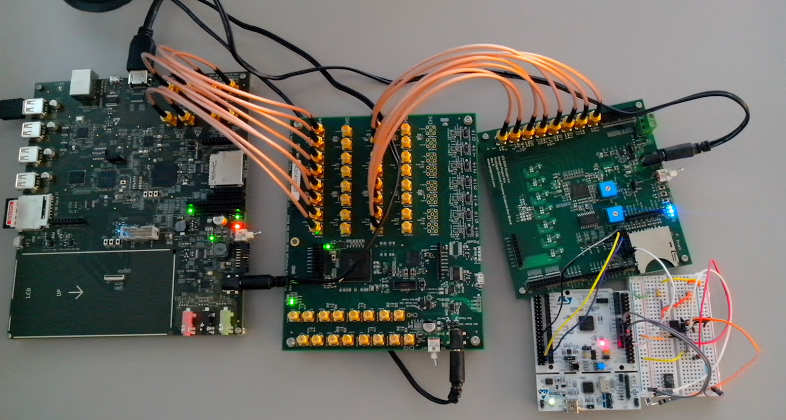
\includegraphics{Pictures/receiver_setup.jpg}
    }}
    \rule{35em}{0.5pt}
  \caption[The ARA MDK and its VLC receiver module]{The ARA MDK and its VLC receiver module}
  \label{fig:receiver}
\end{figure}

\subsection{Circuit Evaluation}

The received signal was measured at different step of the analogical processing, using the 2 oscilloscope voice at different point of our circuit.

\begin{figure}[htbp]
	\centering
	\makebox[\textwidth][c]{
		\scalebox{0.6}{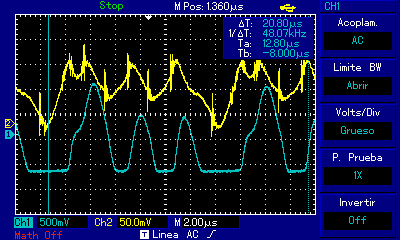
\includegraphics{Pictures/circuit-compare.png}
	}}
		\rule{35em}{0.5pt}
		\caption[In yellow the signal just after the TIA. In blue, the signal after analogical filtering - 2,5 meter distance]{In yellow the signal just after the TIA. In blue, the signal after analogical filtering - 2,5 meter distance}
		\label{fig:circuit-compare}
	\end{figure}
	
\subsection{Digitalization and demodulation}


\subsection{Bit Error Rate}

The BER, just before 4B6B decoding, was computed for different illumination level and clock-rate.

\begin{table}[htbp]
\begin{center}
\begin{tabular}{|c|c|c|}
  \hline
  clock rate (kHz) & bitrate (kbps) & BER \\
  \hline
  100 & 67 & $<$ 10$^6$ \\
  160 & 107 & $<$ 10$^6$ \\
  240 & 160 & 6.10$^4$ \\
  380 & 253 & 3.10$^3$ \\
  560 & 373 & 2.10$^2$ \\
  \hline
\end{tabular}
\end{center}
\caption{Bit Error Rate for different clock frequency at 2,5 meters}
\label{tab:ber}
\end{table}

Considering table \ref{tab:ber} 2,5 meters distance and 10$^-3$ as admissible BER, we can assume that using a 380kHz clock rate can be used for a correct transmission. 

In that case, with 4B6B coding, we obtain a raw throughput of 253 kbps. 
%----------------------------------------------------------------------------------------
%	RESULTS AND INTERPRETATION-----------------------

%-----------------------------------------------------------------
\section{Results and interpretations}

Comparing our result with \citep{phycomp}, we can increase the 
\subsection{Results}
\subsection{Interpretation}